\section{Model Definition}
\label{sec:model}
We model religious affiliation as a multi-strain, contact-driven diffusion process in which religions compete for adherents. The epidemiological analogy specifies transition mechanisms; it does not identify religious belief with pathology. The model combines role heterogeneity, cross-affiliation conversion, demographic turnover, and missionary relabeling representing schism within a fixed set of potential religions \cite{lazebnik2022generic,shami2022economic}. Unlike classical SIR, disaffiliation returns individuals to a susceptible state, and there is no permanently recovered compartment. Figure~\ref{fig:model_scheme} summarizes the transitions.

\begin{figure}[!htbp]
\centering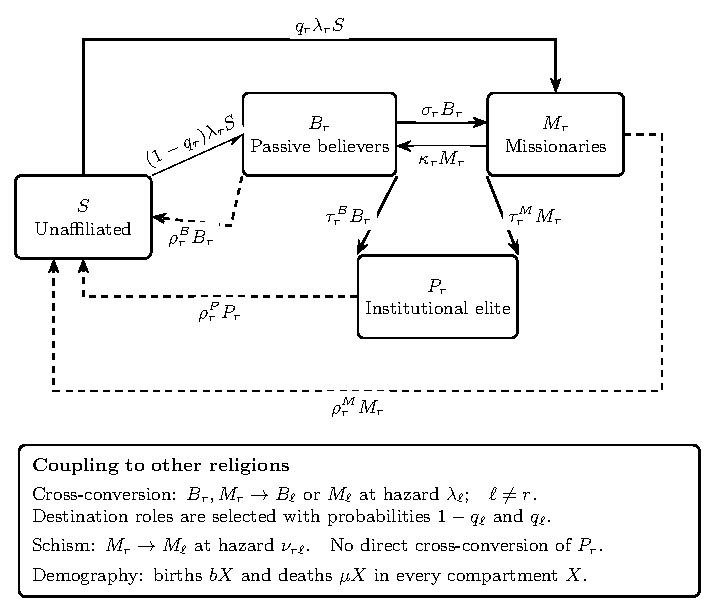
\includegraphics[width=.94\linewidth]{scheme.pdf}
\caption{Role-structured transitions for a focal religion $r$. Conversion is generated by missionaries; a new convert enters $B_r$ with probability $1-q_r$ or $M_r$ with probability $q_r$. Cross-conversion and missionary relabeling couple this structure to the other religions, as specified below the diagram. Births and deaths apply to every compartment.}
\label{fig:model_scheme}
\end{figure}

Let $\mathcal R=\{1,\ldots,m\}$ be a fixed set of modeled religions; some may initially be absent. Each person occupies exactly one state: $S$ (unaffiliated), $B_r$ (affiliated but not actively proselytizing), $M_r$ (actively proselytizing), or $P_r$ (an institutional or religious elite protected from direct cross-conversion). Thus
\begin{equation}
N(t)=S(t)+\sum_{r=1}^m[B_r(t)+M_r(t)+P_r(t)].
\end{equation}
The model excludes simultaneous affiliations. The distinction between $B_r$, $M_r$, and $P_r$ is behavioral and institutional, not a measured distinction in the historical datasets used below.

Under homogeneous mixing, the force of conversion to religion $r$ is
\begin{equation}
\lambda_r(t)=\beta_r(t)\frac{M_r(t)}{N(t)},\qquad
X_r(t)=S(t)+\sum_{j\ne r}[B_j(t)+M_j(t)].
\label{eq:force}
\end{equation}
Here $\beta_r$ is an effective contact-and-conversion rate per missionary, not a probability conditional on a measured contact. All continuous-time rates have units year$^{-1}$; $q_r\in[0,1]$ is dimensionless. Conversion into religion $r$ occurs at rate $\lambda_rX_r$ and is divided between $B_r$ and $M_r$ with weights $1-q_r$ and $q_r$. Each $B_r$ and $M_r$ individual faces an outward cross-conversion hazard $\sum_{\ell\ne r}\lambda_\ell$. Priests do not directly generate conversions and cannot be directly converted to another religion, although they may disaffiliate.

Within an affiliation, $\sigma_r$ governs $B_r\to M_r$, $\kappa_r$ governs $M_r\to B_r$, and $\tau_r^B,\tau_r^M$ govern progression into $P_r$. Disaffiliation from role $X\in\{B,M,P\}$ occurs at rate $\rho_r^X$. Missionary relabeling from $r$ to $\ell$ occurs at rate $\nu_{r\ell}\geq0$, with $\nu_{rr}=0$. This transfers an existing individual from $M_r$ to $M_\ell$; it does not create a person or an additional equation. It represents entry into a previously specified denomination, rather than unrestricted innovation of new labels.

Births and deaths occur at rates $bX$ and $\mu X$ in every compartment $X$. This composition-preserving assumption is a demographic bookkeeping approximation: it does not assert that newborns literally become missionaries or priests. It implies $\dot N=(b-\mu)N$. Uniform demographic growth cancels from the deterministic equations for population fractions, although demographic sampling contributes finite-population variation in the stochastic implementation.

The resulting ODE system is
\begin{align}
\dot S&=(b-\mu)S-S\sum_k\lambda_k+
 \sum_k(\rho_k^BB_k+\rho_k^MM_k+\rho_k^PP_k),\label{eq:S-dynamics}\\
\dot B_r&=(b-\mu)B_r+(1-q_r)\lambda_r X_r-B_r\sum_{\ell\ne r}\lambda_\ell
 -\sigma_rB_r+\kappa_rM_r-(\rho_r^B+\tau_r^B)B_r,\label{eq:B-dynamics}\\
\dot M_r&=(b-\mu)M_r+q_r\lambda_rX_r-M_r\sum_{\ell\ne r}\lambda_\ell
 +\sigma_rB_r-(\kappa_r+\rho_r^M+\tau_r^M)M_r\nonumber\\
&\quad+\sum_{\ell\ne r}\nu_{\ell r}M_\ell-\sum_{\ell\ne r}\nu_{r\ell}M_r,\label{eq:M-dynamics}\\
\dot P_r&=(b-\mu)P_r+\tau_r^BB_r+\tau_r^MM_r-\rho_r^PP_r.\label{eq:P-dynamics}
\end{align}
All transfers are nonnegative at the boundary of the state space, so nonnegative initial states remain nonnegative. Summing the equations cancels conversion, role changes, disaffiliation, and mutation. In particular, an absent religion with no incoming missionary relabeling and no external introduction remains absent. This property supplies a useful implementation check and distinguishes endogenous seeding from imposed introductions.

\paragraph{Optional contextual modulation.}
To make the proposed connection to external conditions explicit, a positive-rate extension is
\begin{equation}
\beta_r(t)=\beta_{r,0}\exp\{\boldsymbol\eta_r^\mathsf{T}\mathbf z_r(t)\},
\label{eq:context}
\end{equation}
where $\mathbf z_r(t)$ contains specified social, institutional, or political covariates and $\boldsymbol\eta_r$ their coefficients. The implementation accepts supplied covariate series, with linear interpolation between supplied times. This extension is motivated by context-sensitive social-epidemiological modeling \cite{emit_paper}; it is not estimated or empirically tested here. The experiments instead use constant rates, or explicitly prescribed piecewise-constant rates in Scenario B and the reduced Sweden fit. No measured political effect, or causal interpretation of a fitted rate change, is claimed.

\paragraph{Role of the historical reduction.}
For a single religion, setting $B=P=0$, $q=1$, all role-transition rates and mutation to zero, and $y=M/N$ gives exactly
\begin{equation}
\dot y=\beta(t)y(1-y)-\rho(t)y.
\label{eq:histfit_reduced_ode}
\end{equation}
These restrictive assumptions remove the mechanisms that distinguish the full model. More generally, $\dot y$ depends on the unobserved missionary share and role-specific losses, so aggregate affiliation alone does not close the full system. We therefore use Eq.~\eqref{eq:histfit_reduced_ode} as a descriptive reduced benchmark, not as empirical validation of role heterogeneity, competition, or schism. For publisher activity and no-religion reporting, its coefficients are phenomenological rather than literal missionary conversion and apostasy rates.
